% !TeX program = xelatex
\documentclass{sbc2023}

\usepackage{graphicx}
\usepackage[misc,geometry]{ifsym}
\usepackage{fontspec}
\usepackage{fontawesome}
\usepackage{academicons}
\usepackage{color}
\usepackage{xcolor}
\usepackage{hyperref}
\usepackage{aas_macros}
\usepackage[bottom]{footmisc}
\usepackage{supertabular}
\usepackage{afterpage}
\usepackage{url}
\usepackage{pifont}
\usepackage{multicol}
\usepackage{multirow}
\usepackage{booktabs}
\usepackage{tabularx}
\usepackage{array}
\usepackage{amsmath}
\usepackage{enumitem}
\usepackage{seqsplit}
\usepackage[section]{placeins}
\usepackage{balance}
\usepackage{tikz}
\usetikzlibrary{arrows.meta,positioning}

\setcitestyle{square}
\definecolor{darkblue}{rgb}{0.0,0.0,0.0}
\definecolor{berrybrand}{HTML}{CC4168}
\definecolor{leafbrand}{HTML}{96B55C}
\definecolor{orcidlogo}{rgb}{0.37,0.48,0.13}
\hypersetup{
  colorlinks=true,
  linkcolor=darkblue,
  citecolor=darkblue,
  urlcolor=darkblue,
  pdftitle={BerryBrain: Architecture and Experimental Evaluation},
  pdfauthor={Mateus Almeida de Souza and Leonardo José Silvestre}
}

\newcommand{\BerryBrain}{\textit{BerryBrain}}
\newcommand{\NA}{\textit{n/a}}
\newcommand{\CI}{95\% CI}
\newcommand{\code}[1]{\texttt{#1}}
\newcolumntype{Y}{>{\raggedright\arraybackslash}X}
\setlist{nosep,leftmargin=*}
\setlist[description]{nosep,leftmargin=1.2cm,labelwidth=1cm,labelsep=0.2cm}
\setlength{\emergencystretch}{1em}
\setlength{\vfuzz}{2pt}

\jid{}
\jtitle{\strut}
\doi{}
\copyrightstatement{}
\jyear{2026}

\title[BerryBrain: Architecture and Experimental Evaluation]{BerryBrain: Architecture and Experimental Evaluation of an Adaptive Knowledge Management System Based on Semantic Graphs, GraphRAG, and Human Feedback}

\author[Souza and Silvestre 2026]{
\affil{\textbf{Mateus Almeida de Souza}~\href{https://orcid.org/0009-0000-4701-1282}{\textcolor{orcidlogo}{\aiOrcid}}~\textcolor{blue}{\faEnvelopeO}~~[~\textbf{UFES/CEUNES, São Mateus, Brazil}~|~\href{mailto:mateus.a.souza@edu.ufes.br}{\textbf{\textit{mateus.a.souza@edu.ufes.br}}}~]}
\affil{\textbf{Leonardo José Silvestre}~\textcolor{blue}{\faEnvelopeO}~~[~\textbf{UFES/CEUNES, São Mateus, Brazil}~|~\href{mailto:leonardo.silvestre@ufes.br}{\textbf{\textit{leonardo.silvestre@ufes.br}}}~]}
}

\begin{document}

\begin{frontmatter}
\maketitle

\begin{mail}
Department of Computing and Electronics, Northern Espírito Santo University Center,
Federal University of Espírito Santo, São Mateus, Espírito Santo, Brazil.
\end{mail}

\begin{abstract}
\textbf{Abstract.~}
Personal knowledge management systems preserve notes under user control, but they often rely on
manual links and lexical retrieval. Retrieval-augmented generation improves access to stored
knowledge, yet purely vector-based approaches may miss cross-document relationships and generate
answers whose provenance is difficult to audit. This work presents \BerryBrain, a self-hosted
system that converts Markdown notes into a governed semantic graph, combines lexical, dense, and
structural retrieval through GraphRAG, and incorporates provenance, confidence estimates, a
configurable panel of language-model judges, and reversible human feedback. The study follows
Design Science Research and evaluates version 1.4.8 through automated tests, paired retrieval
ablation, a public benchmark, and performance, fault, security, accessibility, and maturity
assessments. On a controlled 44-query fixture, graph-hybrid retrieval achieved Recall@10 of 1.00,
compared with 0.50 for hybrid retrieval without graph expansion. On 20 multi-hop queries, the
difference was 1.00 with an exploratory bootstrap interval of [1.00, 1.00]. This result validates
the intended regression behavior, not external superiority. On BEIR SciFact, an independent BM25
implementation achieved Recall@10 of 0.7816, MRR of 0.6386, and nDCG@10 of 0.6644 over 300
queries. API statement coverage reached 82.19\%, and Worker coverage reached 48.94\%; 465 API
tests, 55 Worker tests, and 56 end-to-end scenarios passed. On a Raspberry Pi 4, the API sustained
62.02 requests/s at 274.36 ms p95, while a synthetic 10,000-node graph completed loading in
6.35 s. The
evaluation supports architectural coherence and regression behavior but does not yet validate
human calibration of the judges, semantic generalization, or longitudinal learning from users.
The work contributes an auditable architecture, an edit-and-delete lifecycle, and a reproducible
protocol that distinguishes non-parametric adaptation from model-weight training.
\end{abstract}

\begin{keywords}
personal knowledge management, personal knowledge graph, GraphRAG, information retrieval,
provenance, LLM as a judge, human feedback, self-hosted systems
\end{keywords}

\end{frontmatter}

\section{Introduction}
\label{sec:intro}

Personal notes record decisions, readings, hypotheses, and experience, but their value depends on
the ability to retrieve not only documents but also relationships, contradictions, and knowledge
gaps. Personal knowledge management (PKM) supports this process, while personal knowledge graphs
(PKGs) formalize entities and relationships controlled by an individual
\cite{balog2019pkg,chakraborty2023survey,skjaeveland2024ecosystem}. Recent systems use natural
language processing to suggest connections between notes \cite{fraga2023automatic,
fraga2024connections}, but governance, provenance, update semantics, and evaluation remain open
problems.

Retrieval-augmented generation (RAG) conditions language models on external evidence
\cite{lewis2020rag}. Dense retrievers are effective at semantic similarity
\cite{karpukhin2020dpr}, but fragment similarity alone does not represent paths across sources.
GraphRAG adds relational structure, communities, and corpus-level summaries
\cite{edge2024graphrag}; HippoRAG models associative memory \cite{gutierrez2024hipporag}; and
LightRAG proposes incremental graph-vector retrieval \cite{guo2024lightrag}. These advances do not
remove the need to track the origin of every claim, invalidate derivatives when sources change,
or measure the quality of automated evaluators.

The research problem is: \textit{to what extent does an architecture that combines a semantic
graph, hybrid retrieval, multi-agent validation, and explicit feedback improve relevance,
traceability, and knowledge coherence over configurations without graph expansion, and what costs
and limitations does this combination introduce?}

The general objective is to design, implement, and experimentally evaluate an adaptive
architecture that converts personal notes into structured, queryable, and traceable knowledge.
The specific objectives are:

\begin{enumerate}
  \item extract concepts, entities, topics, evidence, and relationships from notes;
  \item build a graph with governed classes, predicates, provenance, and lifecycle constraints;
  \item integrate lexical, vector, and structural retrieval in a controlled GraphRAG pipeline;
  \item validate and enrich artifacts through rules, agents, and configurable judges;
  \item estimate confidence from observable signals without allowing manual score editing;
  \item incorporate explicit user decisions as auditable and reversible feedback; and
  \item evaluate retrieval, coherence, performance, resilience, security, accessibility, and
  architectural maturity.
\end{enumerate}

This work contributes: (i) a local-first architecture that separates canonical notes from derived
artifacts; (ii) an operational ontology shared by extraction, visualization, and RAG; (iii) an
invalidation protocol for edits and deletions; (iv) feedback-guided non-parametric adaptation; and
(v) a reproducible evaluation that states its evidential limits. The system is not claimed to
learn foundation-model weights. Learning here changes graph state, policies, preferences, and
suppression decisions.

\section{Background and Related Work}
\label{sec:related}

\subsection{Personal knowledge management and graphs}

PKGs organize facts and relationships around one user, with ownership, privacy, and
personalization requirements that differ from enterprise knowledge graphs
\cite{balog2019pkg}. Recent surveys identify graph population, interoperability, utilization, and
evaluation as open issues \cite{chakraborty2023survey,skjaeveland2024ecosystem}. Fraga et al.
\cite{fraga2024connections} demonstrate automatic PKM connections and provide the closest
peer-reviewed comparator for note linking. \BerryBrain extends this scope by treating admission,
provenance, lifecycle, structural retrieval, and feedback as one contract.

\subsection{RAG, GraphRAG, and multi-hop retrieval}

RAG integrates retrieval and generation \cite{lewis2020rag}. BM25 remains a strong lexical
baseline across heterogeneous collections, as shown by BEIR \cite{thakur2021beir}. Dense passage
retrieval learns query and passage representations \cite{karpukhin2020dpr}, while Reciprocal Rank
Fusion combines ranked lists without requiring comparable score scales
\cite{cormack2009rrf}. Multi-hop datasets such as HotpotQA and MuSiQue require evidence composition
across sources \cite{yang2018hotpotqa,trivedi2022musique}.

GraphRAG constructs relationships and communities for local and global questions
\cite{edge2024graphrag}. HippoRAG uses graphs and personalized PageRank for associative retrieval
\cite{gutierrez2024hipporag}. HippoRAG 2 deepens passage integration and frames external memory as
non-parametric continual learning across factual, sense-making, and associative tasks
\cite{gutierrez2025hipporag2}. LightRAG separates low- and high-level retrieval and emphasizes
incremental updates \cite{guo2024lightrag}. This work does not claim universal superiority over
these systems; it evaluates an integrated artifact and uses internal ablations to isolate
structural expansion.

\subsection{RAG evaluation and LLM as a judge}

RAGAS measures faithfulness and relevance without always requiring textual references
\cite{es2024ragas}; ARES combines synthetic data, human annotations, and statistical inference
\cite{saadfalcon2024ares}. LLM evaluators may align with human preferences, but they are not
oracles \cite{liu2023geval}. Specialized evaluators \cite{kim2024prometheus} and position bias
\cite{shi2025judges} reinforce the need for calibration against independent human reviewers.

In \BerryBrain, judges receive separate faithfulness, relevance, and contradiction roles. The
active generation model is excluded from the committee by default. Failures remain in provenance
but do not enter voting. This design reduces coupling without turning synthetic agreement into
evidence of human validity.

\subsection{Provenance, ontology, and confidence}

RDF, OWL, SKOS, and PROV-O provide vocabularies for identity, semantics, and provenance
\cite{rdf11,owl2,skos,prov}. \BerryBrain uses a smaller domain-specific operational ontology with
domain and range constraints. Runtime confidence is a bounded summary of observed support signals,
not a calibrated probability of truth. This distinction follows calibration research
\cite{guo2017calibration} and prevents model output from being interpreted as certainty.

\begin{table*}[!t]
\caption{Positioning against related lines of work.}
\label{tab:position}
\small
\begin{tabularx}{\textwidth}{p{2.6cm}YYY}
\toprule
Line & Primary unit & Main strength & Gap addressed in \BerryBrain \\
\midrule
PKG/PKM & personal notes, entities, and links & ownership and organization & lifecycle, feedback, and integrated evaluation \\
Vector RAG & semantically similar fragments & semantic retrieval & multi-hop relations and structural provenance \\
GraphRAG & entities, edges, and communities & corpus-level sense-making & local-first governance and source invalidation \\
LLM as a judge & automated verdicts & scalable evaluation & configurable committee, failure records, and explicit calibration \\
\bottomrule
\end{tabularx}
\end{table*}
\FloatBarrier

\section{Research Method}
\label{sec:method}

\subsection{Research strategy}

The study follows Design Science Research Methodology (DSRM), whose activities comprise problem
identification, solution objectives, design and development, demonstration, evaluation, and
communication \cite{hevner2004design,peffers2007dsrm}. The artifact is \BerryBrain 1.4.8. Its
design principles are treated as knowledge contributions only to the extent supported by the
reported evidence.

This is an exploratory engineering evaluation. It used no human participants, personal note
content, or model training. Deterministic fixtures exercised internal contracts, while BEIR
SciFact supplied a public external reference for BM25. The confirmatory phase includes an
annotated corpus, blinded human reviewers, and a longitudinal study; no values were simulated for
those pending studies.

\subsection{Research questions}

\begin{description}
  \item[RQ1:] Does graph expansion improve multi-hop retrieval without an observed factual loss?
  \item[RQ2:] Do ontology, provenance, and judge controls block unsupported claims and stale evidence?
  \item[RQ3:] Do creation, editing, and deletion preserve graph coherence?
  \item[RQ4:] Are evidence-support estimates signal-derived and auditable, and are they calibrated against correctness?
  \item[RQ5:] Is the judge committee regression-stable and aligned with human reviewers?
  \item[RQ6:] What latency, memory, payload, queue, and frontend costs are introduced?
  \item[RQ7:] Does the system improve human tasks over search and non-graph RAG?
  \item[RQ8:] Does explicit feedback reduce recurrence of rejected artifacts?
  \item[RQ9:] Does the system preserve state and recover from failures?
\end{description}

\subsection{Comparative design}

Four layers prevent invalid comparisons. Internal ablation keeps corpus, qrels, order, context
limit, and cache policy fixed while varying lexical, dense, hybrid, and graph expansion.
Independent technical baselines implement BM25, dense retrieval, hybrid retrieval, and vanilla RAG
on the same corpus. Historical regression compares frozen revisions. User studies compare complete
workflows and require an approved ethics protocol. Only the first layer and an external BM25
implementation check were executed in this stage.

Retrieval metrics were Recall@10, MRR, and nDCG@10. Generation and graph outcomes included citation
support, unsupported claims, ontology violations, stale residue, and idempotence. Performance
outcomes included median, p95, p99, throughput, peak memory, and payload. The exploratory paired
interval used percentile bootstrap with 2,000 resamples and seed 20260812. Confirmatory execution
requires at least 10,000 resamples, a preregistered non-inferiority margin, and Holm correction
\cite{efron1993bootstrap,holm1979procedure}.

\subsection{Environment and reproducibility}

The principal verification and integrated benchmark reruns occurred on August 24, 2026 in
\code{America/Sao\_Paulo}, producing UTC artifacts on August 25. Their benchmark manifest records
release revision \code{a81c566} (tag \code{v1.4.8}) plus a dirty worktree, which remains a
limitation. Hardware was a Raspberry Pi 4 with four ARM Cortex-A72 cores up to 1.8 GHz and
7.6 GiB RAM, running Debian aarch64 and Linux 6.12.62. The host exposed Python 3.11.2, while the
integrated benchmark environment recorded Python 3.13.13; Node.js was 20.20.2 and Docker was
29.3.1. A historical mismatch between Python package metadata and module constants was corrected
to 1.4.8 and retested.

The implementation uses Python \cite{python}, FastAPI, Pydantic, and SQLAlchemy in the API
\cite{fastapi,pydantic,sqlalchemy}; Next.js and React in the frontend \cite{nextjs,react}; and
Docker for orchestration \cite{docker}. Testing and analysis use pytest, Playwright, Ruff, and uv
\cite{pytest,playwright,ruff,uv}. These citations point to primary software documentation;
resolved versions and lockfiles remain the reproducibility authority.

\begin{table*}[!t]
\caption{Software stack observed during evaluation.}
\label{tab:stack}
\small
\begin{tabularx}{\textwidth}{p{2.8cm}p{3.4cm}Y}
\toprule
Layer & Tools and versions & Role \\
\midrule
API & Python 3.11.2; FastAPI 0.140.0; SQLAlchemy 2.0.51; Pydantic 2.13.4 & HTTP, domain logic, validation, and persistence \\
Frontend & Next.js 15.5.22; React 19.2.7 & web interface and rendering \\
End-to-end & Playwright 1.61.1 / Chromium & workflows, accessibility, and performance \\
Packaging & Docker 29.3.1 & service and build isolation \\
Build and quality & uv 0.5.9; pytest; Ruff; MyPy & dependencies, tests, and static analysis \\
\bottomrule
\end{tabularx}
\end{table*}

\begin{table*}[!t]
\caption{Executed evidence sources.}
\label{tab:evidence}
\small
\begin{tabularx}{\textwidth}{p{3.2cm}p{2.1cm}Y}
\toprule
Source & Scale & Purpose \\
\midrule
Semantic fixture & 100 notes, 45 queries & retrieval, negative queries, and latency \\
Retrieval ablation & 44 queries & 20 multi-hop, 20 factual, and 4 negative \\
Cognitive fixture & 6 notes & extraction, connections, insights, provenance, and lifecycle \\
BEIR SciFact & 5,183 docs, 300 queries & public independent BM25 reference \\
Synthetic graph & 5k/20k and 10k nodes & backend, payload, memory, and rendering \\
Worker queue & 100 jobs & enqueue, drain, claim, and duplication \\
Local HTTP & 100 requests, concurrency 10 & throughput and latency percentiles \\
Browser & 5 repetitions per route/device & LCP, CLS, long tasks, and transfer \\
\bottomrule
\end{tabularx}
\end{table*}
\FloatBarrier

\subsection{Ethics, privacy, and AI use}

No participant data or personal notes were collected. Fixtures are not loaded during production
startup. The project separates canonical vault content, derived indexes, and telemetry; exports
redact secrets. A future user study must be submitted to the applicable research ethics committee
and include consent, data minimization, retention, and withdrawal procedures.

Generative AI tools assisted software engineering, code review and debugging, the design and
addition of automated tests, research organization, manuscript structure, and language revision.
They did not autonomously establish the reported evidence or conclusions. The first author executed
the test suites, inspected the retained outputs, and verified metrics, code, sources, and claims.
Both authors retain full responsibility for the manuscript. No AI system is listed as an author. This
disclosure follows the transparency and accountability requirements of the Brazilian Computer
Society publication policy.

\section{The BerryBrain Artifact}
\label{sec:artifact}

\subsection{Architecture}

\BerryBrain is local-first: Markdown notes remain the user-controlled canonical content, while
stable identities, provenance, feedback policy, settings, and job state form authoritative
operational control data. Generated graph records, lexical and vector indexes, the HippoRAG
projection, and caches are derived and rebuildable. The runtime comprises a Next.js frontend, a
FastAPI service, an asynchronous Worker, SQLite, an optional HippoRAG sidecar, and one active local
or cloud model route. Local-first therefore describes ownership and recoverability; it does not
imply that every inference executes locally.

\begin{figure*}[!t]
\centering
\resizebox{0.98\textwidth}{!}{%
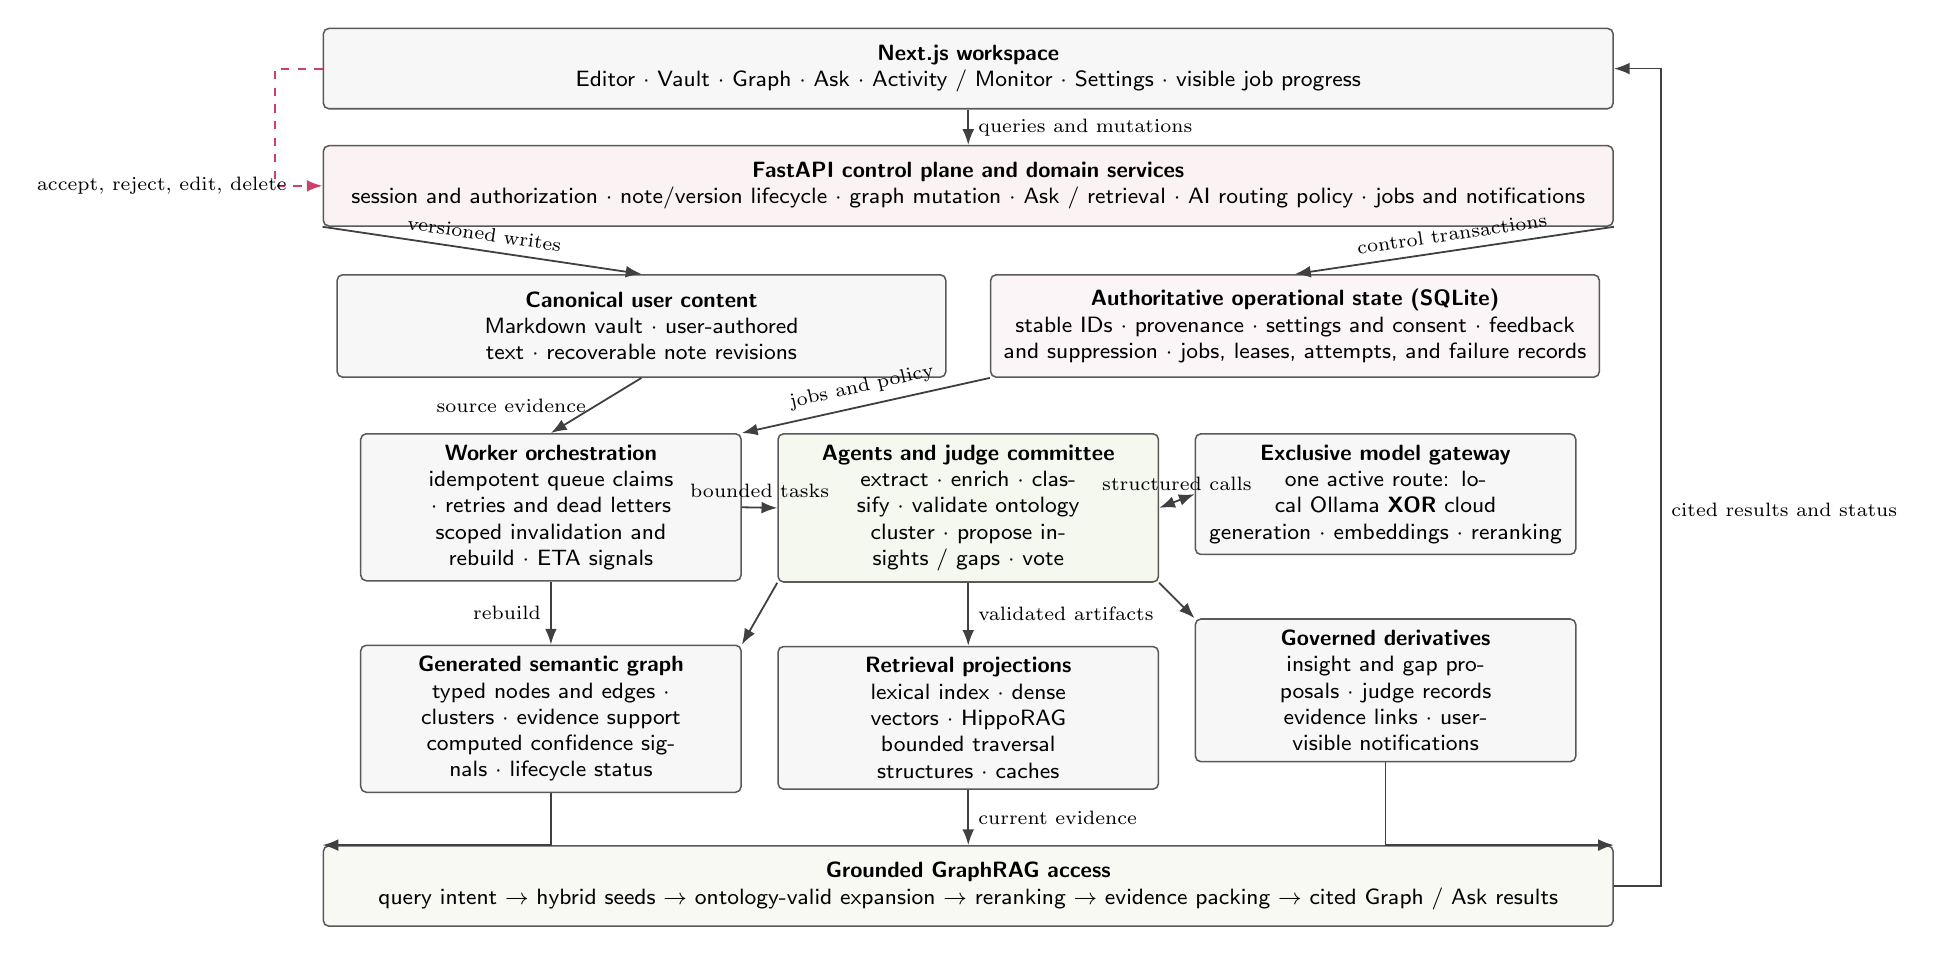
\begin{tikzpicture}[
  font=\sffamily\footnotesize,
  wide/.style={draw=black!65, line width=0.55pt, rounded corners=2pt,
    align=center, text width=16.1cm, minimum height=1.02cm, inner sep=4pt},
  pair/.style={draw=black!65, line width=0.55pt, rounded corners=2pt,
    align=center, text width=7.45cm, minimum height=1.30cm, inner sep=4pt},
  module/.style={draw=black!65, line width=0.55pt, rounded corners=2pt,
    align=center, text width=4.55cm, minimum height=1.48cm, inner sep=4pt},
  flow/.style={-{Latex[length=2mm]}, draw=black!75, line width=0.65pt},
  exchange/.style={{Latex[length=2mm]}-{Latex[length=2mm]}, draw=black!75,
    line width=0.65pt},
  feedback/.style={-{Latex[length=2mm]}, draw=berrybrand, dashed, line width=0.75pt}
]
\node[wide, fill=black!3] (ui) {\textbf{Next.js workspace}\\
Editor $\cdot$ Vault $\cdot$ Graph $\cdot$ Ask $\cdot$ Activity / Monitor
$\cdot$ Settings $\cdot$ visible job progress};
\node[wide, fill=berrybrand!7, below=4.5mm of ui] (api) {\textbf{FastAPI control plane and domain services}\\
session and authorization $\cdot$ note/version lifecycle $\cdot$ graph mutation
$\cdot$ Ask / retrieval $\cdot$ AI routing policy $\cdot$ jobs and notifications};

\node[pair, fill=black!3, below=6mm of api, xshift=-4.15cm] (vault) {\textbf{Canonical user content}\\
Markdown vault $\cdot$ user-authored text $\cdot$ recoverable note revisions};
\node[pair, fill=berrybrand!5, below=6mm of api, xshift=4.15cm] (state) {\textbf{Authoritative operational state (SQLite)}\\
stable IDs $\cdot$ provenance $\cdot$ settings and consent $\cdot$ feedback and suppression
$\cdot$ jobs, leases, attempts, and failure records};

\node[module, fill=black!3, below=7mm of vault, xshift=-1.15cm] (worker) {\textbf{Worker orchestration}\\
idempotent queue claims $\cdot$ retries and dead letters\\
scoped invalidation and rebuild $\cdot$ ETA signals};
\node[module, fill=leafbrand!10, below=7mm of vault, xshift=4.15cm] (agents) {\textbf{Agents and judge committee}\\
extract $\cdot$ enrich $\cdot$ classify $\cdot$ validate ontology\\
cluster $\cdot$ propose insights / gaps $\cdot$ vote};
\node[module, fill=black!3, below=7mm of state, xshift=1.15cm] (models) {\textbf{Exclusive model gateway}\\
one active route: local Ollama \textbf{XOR} cloud\\
generation $\cdot$ embeddings $\cdot$ reranking};

\node[module, fill=black!3, below=8mm of worker] (graph) {\textbf{Generated semantic graph}\\
typed nodes and edges $\cdot$ clusters $\cdot$ evidence support\\
computed confidence signals $\cdot$ lifecycle status};
\node[module, fill=black!3, below=8mm of agents] (indexes) {\textbf{Retrieval projections}\\
lexical index $\cdot$ dense vectors $\cdot$ HippoRAG\\
bounded traversal structures $\cdot$ caches};
\node[module, fill=black!3, below=8mm of models] (proposals) {\textbf{Governed derivatives}\\
insight and gap proposals $\cdot$ judge records\\
evidence links $\cdot$ user-visible notifications};

\node[wide, fill=leafbrand!8, below=7mm of indexes] (retrieval) {\textbf{Grounded GraphRAG access}\\
query intent $\rightarrow$ hybrid seeds $\rightarrow$ ontology-valid expansion
$\rightarrow$ reranking $\rightarrow$ evidence packing $\rightarrow$ cited Graph / Ask results};

\draw[flow] (ui) -- node[right, font=\scriptsize]{queries and mutations} (api);
\draw[flow] (api.south west) -- node[above, sloped, font=\scriptsize]{versioned writes} (vault.north);
\draw[flow] (api.south east) -- node[above, sloped, font=\scriptsize]{control transactions} (state.north);
\draw[flow] (vault.south) -- node[left, font=\scriptsize]{source evidence} (worker.north);
\draw[flow] (state.south west) -- node[above, sloped, font=\scriptsize]{jobs and policy} (worker.north east);
\draw[flow] (worker.east) -- node[above, font=\scriptsize]{bounded tasks} (agents.west);
\draw[exchange] (agents.east) -- node[above, font=\scriptsize]{structured calls} (models.west);
\draw[flow] (worker.south) -- node[left, font=\scriptsize]{rebuild} (graph.north);
\draw[flow] (agents.south west) -- (graph.north east);
\draw[flow] (agents) -- node[right, font=\scriptsize]{validated artifacts} (indexes);
\draw[flow] (agents.south east) -- (proposals.north west);
\draw[flow] (graph.south) |- (retrieval.north west);
\draw[flow] (indexes) -- node[right, font=\scriptsize]{current evidence} (retrieval);
\draw[flow] (proposals.south) |- (retrieval.north east);
\draw[flow] (retrieval.east) -- ++(6mm,0) |- node[pos=0.23,right, font=\scriptsize]{cited results and status} (ui.east);
\draw[feedback] (ui.west) -- ++(-6mm,0) |- node[pos=0.73,left, font=\scriptsize]{accept, reject, edit, delete} (api.west);
\end{tikzpicture}%
}
\caption{BerryBrain runtime, authority, and adaptation boundaries. Solid arrows show transactional,
job, model, artifact, or retrieval flow; the dashed arrow shows auditable user feedback and
lifecycle actions. Markdown is canonical user content, SQLite retains authoritative control state,
and graph, retrieval, and proposal structures are derived and rebuildable.}
\label{fig:architecture}
\end{figure*}
\FloatBarrier

Cloud providers and Ollama are mutually selected runtime modes. The active configuration determines
the route; local calls must not occur while cloud mode is active. Jobs expose status, attempts,
failure reasons, and operational estimates. Autopilot schedules enrichment, insights, gaps, judge
evaluation, and clustering without requiring manual feature buttons.

\subsection{Operational ontology}

The ontology prevents the graph from becoming a visualization of arbitrary words. Each class has
a meaning, visual shape, and naming rules. Each predicate is a directed verb phrase with domain,
range, symmetry, and admissible evidence. Navigation fragments, isolated verbs, stop phrases,
unsupported abbreviations, and diagnostics are rejected or quarantined.

\begin{table}[!htbp]
\caption{Canonical node classes.}
\label{tab:nodes}
\centering
\scriptsize
\begin{tabularx}{\columnwidth}{p{1.48cm}p{0.98cm}Y}
\toprule
Class & Shape & Semantics \\
\midrule
Note & circle & canonical document and provenance root \\
Concept & diamond & reusable abstract idea expressed by sources \\
Entity & hexagon & identifiable person, organization, place, product, event, or work \\
Topic & triangle & broad thematic group for navigation and retrieval \\
Insight & rectangle & evidence-supported proposal subject to acceptance \\
Research\allowbreak Gap & octagon & unresolved question or missing evidence \\
\bottomrule
\end{tabularx}
\end{table}
\FloatBarrier

Shape encodes class; color encodes semantic cluster; color never encodes confidence. Every current
cluster receives a deterministic contrast-safe color. A parent note uses the primary
\code{\#CC4168} color, and insights receive a highlight while remaining rectangular. Canonical
predicates include \code{mentions}, \code{defines}, \code{supports}, \code{contradicts},
\code{broaderThan}, \code{narrowerThan}, \code{relatedTo}, \code{derivedFrom}, and
\code{evidencedBy}. The machine-readable contract validates permitted endpoints before admission.

\subsection{Retrieval and grounded answers}

Ask accepts questions about graph content and graph topology. The pipeline retrieves lexical and
dense seeds, applies fusion, expands only ontology-valid paths, removes stale or suppressed
sources, reranks with conservative support, and passes cited evidence to the generator. If a
provider fails, the interface does not display an answer-like fallback. It preserves a waiting or
error state and offers retry and configuration actions. Question suggestions are generated only
when relevant graph content exists.

\subsection{Signal-derived evidence-support interval}

Clients cannot write confidence. Given distinct normalized signals $x_i\in[0,1]$, the runtime
computes their mean $\bar{x}$ and a nominal two-sided, empirical-Bernstein-style bounded interval.
The implementation follows the radius form of Audibert et al. \cite{audibert2009exploration},
uses the Bessel-corrected sample variance $s^2$, and fixes the nominal level at $1-\delta=0.95$.
For $n>1$:

\begin{equation}
\begin{aligned}
r&=\sqrt{\frac{2s^2\ln(3/\delta)}{n}}+
\frac{3\ln(3/\delta)}{n},\\
L&=\max(0,\bar{x}-r),\\
U&=\min(1,\bar{x}+r).
\end{aligned}
\end{equation}

Bounds are clipped to $[0,1]$. The displayed score is the midpoint $(L+U)/2$ of those clipped
bounds; downstream ranking may use $L$ conservatively. One scored signal deliberately yields
$[0,1]$, and no scored observations yield an unavailable state. Provenance identifiers remain
listed as factors but do not increase $n$, avoiding one form of double-counting. The serialized
method is \code{empirical-bernstein-bounded-signals-v1}.

The theoretical concentration guarantee assumes bounded independent observations estimating a
common expectation. BerryBrain combines heterogeneous heuristic, model, and user signals whose
sampling process has not been validated against those assumptions. Consequently, ``95\%'' is a
nominal construction level and the output is an \emph{evidence-support uncertainty interval}, not
a frequentist coverage claim for factual truth and not a calibrated correctness probability. This
runtime interval is also distinct from the paired percentile bootstrap used for retrieval effects.

\subsection{Feedback and lifecycle}

Semantically meaningful actions generate append-only learning events. Creating or materially
editing a note schedules a new version and detaches obsolete provenance when required. Renaming or
moving preserves identity. Deletion removes note-owned evidence and recalculates only dependent
neighborhoods. Confirming, ignoring, correcting, restoring, or deleting a node or edge updates an
active policy by canonical identity and source scope. Accepting or rejecting an insight and
correcting an Ask answer also produce policy signals. Navigation and incidental clicks are not
learning labels.

Before deleting a derived node, the API captures incident edges, sources, neighbors, cluster, and
dependent insights. Within the transaction, it expires insights, quarantines relationships that
cite the artifact, removes projections, and records negative feedback. It then schedules scoped
relationship reconciliation, insight rediscovery, judging, and reclustering. Consequently, a
rejected identity must not silently reappear after refresh, and relationships that depended on it
must not remain active.

\subsection{Agents and judge committee}

Agents propose extraction, enrichment, connections, clusters, insights, gaps, and answers; they do
not directly admit knowledge. Deterministic validators enforce type, naming, provenance, state,
and ontology rules. Judges assess faithfulness, relevance, contradiction, source quality, and
ontology consistency.

The committee discovers the live provider catalog and sends structured probes through the same
runtime route. Embedding, reranking, moderation, audio, image, and active generator models are
excluded. Each slot persists provider, model, role, and focus and remains editable in Settings.
The committee requires at least two distinct valid verdicts. Failed calls remain recorded but are
excluded from voting. Catalog presence is insufficient because listed models may still return
404, time out, or reject the required schema.

\section{Experimental Protocol}
\label{sec:protocol}

\subsection{Software verification}

The evaluation executed unit, integration, subtest, Chromium E2E, lint, typecheck, production
build, architecture fitness, security, dependency vulnerability, MyPy, and coverage checks.
Overlapping test counts are not summed as independent observations.

\begin{table*}[!t]
\caption{Executed software verification suites.}
\label{tab:tests}
\small
\begin{tabularx}{\textwidth}{Yrrp{2.5cm}}
\toprule
Suite & Passed & Failed & Note \\
\midrule
API functional & 465 & 0 & 59 subtests \\
API under coverage & 464 & 0 & 1 expected timing skip \\
Worker & 55 & 0 & integrated API import path \\
Chromium E2E & 56 & 0 & 4.1 minutes \\
Focused after fixes & 33 & 0 & benchmark and judge \\
Ruff / MyPy & all & 0 & 6 files in MyPy scope \\
Web lint/typecheck/build & all & 0 & 23 routes, 103 kB shared bundle \\
Architecture fitness & 12 checks & 0 & pass \\
Security audit & 9 checks & 0 & pass \\
\bottomrule
\end{tabularx}
\end{table*}

\subsection{Retrieval ablation}

The fixture includes multi-hop queries intentionally requiring graph paths, factual queries, and
negative queries. Configurations are lexical, dense, standard hybrid, graph lexical, and
graph-hybrid. Because this is a designed regression test, perfect scores only show that the
implementation recovers expected paths.

\subsection{External benchmark}

The official BEIR \code{scifact.zip} archive was downloaded with SHA-256
\texttt{\seqsplit{536e14446a0ba56ed1398ab1055f39fe852686ecad24a6306c80c490fa8e0165}}.
An independent BM25 implementation indexed 5,183 documents and evaluated 300 test queries. This
run verifies the baseline and benchmark infrastructure on public data. The complete BerryBrain
pipeline did not run on the same corpus in this stage, so the numbers do not support a direct
superiority claim. The retained external bundle was generated on August 14 at revision
\code{c297558}; it is reported separately rather than represented as part of the August 25
integrated run.

\subsection{Performance, fault, and frontend tests}

Integrated profile S exercised 5,000 nodes and 20,000 edges over seven samples. An on-disk
benchmark used 500 nodes and 1,000 edges. The queue processed 100 jobs. The HTTP test sent 100
requests at concurrency 10. Fault injection simulated interruption, invalid jobs, and scoped
recomputation while checking containment and state preservation.

Playwright measured public routes on desktop and emulated mobile with five repetitions per cell.
A separate scenario measured 10,000 graph nodes, first visual, complete load, p95 interaction, and
heap. Automated WCAG 2.2 A/AA checks were included, although automation does not replace manual
assessment \cite{wcag22}.

\section{Results}
\label{sec:results}

\subsection{Retrieval quality}

\begin{table}[!htbp]
\caption{Internal ablation over 44 queries (R@10 denotes Recall@10).}
\label{tab:ablation}
\centering
\scriptsize
\setlength{\tabcolsep}{2.5pt}
\begin{tabularx}{\columnwidth}{Yrrrrr}
\toprule
Method & R@10 & MRR & nDCG@10 & p50 ms & p95 ms \\
\midrule
Lexical & 0.05 & 0.0167 & 0.0247 & 7.75 & 9.73 \\
Dense & 0.50 & 0.50 & 0.50 & 7.27 & 8.90 \\
Standard hybrid & 0.50 & 0.50 & 0.50 & 14.94 & 16.69 \\
Graph lexical & 0.50 & 0.25 & 0.3155 & 15.10 & 18.16 \\
Graph-hybrid & \textbf{1.00} & \textbf{0.75} & \textbf{0.8155} & 21.54 & 25.80 \\
\bottomrule
\end{tabularx}
\end{table}

On 20 multi-hop queries, standard hybrid Recall@10 was 0 and graph-hybrid was 1.00; the
difference was 1.00 with an exploratory paired bootstrap \CI\ of [1.00, 1.00]. On 20 factual
queries, both scored 1.00. Citation precision, evidence faithfulness, negative rejection, and stale
evidence removal were 1.00 in the fixture. Graph-hybrid added 9.11 ms at p95 over standard hybrid,
consistent with expansion and reranking.

The separate semantic fixture contained 100 notes and 45 queries. It achieved Recall@5 of 0.50,
Recall@10 of 1.00, MRR and nDCG@10 of 1.00, negative rejection of 1.00, and p95 latency of
45.85 ms. Perfect values reflect deterministic qrels and do not establish generalization.

\begin{table}[!htbp]
\caption{Independent BM25 result on BEIR SciFact.}
\label{tab:beir}
\centering
\small
\begin{tabularx}{\columnwidth}{Yrr}
\toprule
Metric & Result & Scale \\
\midrule
Recall@10 & 0.781611 & 300 queries \\
MRR & 0.638610 & 300 queries \\
nDCG@10 & 0.664390 & 300 queries \\
Index construction & 1,393.12 ms & 5,183 documents \\
p50 / p95 / p99 latency & 309.78 / 386.21 / 406.30 ms & per query \\
\bottomrule
\end{tabularx}
\end{table}

\subsection{Cognitive quality, lifecycle, and judges}

On the six-note cognitive fixture, concept and connection precision and recall were 1.00; grounded
insight and provenance coverage were 1.00; unsupported claims, diagnostic leakage, and stale
artifact rates were zero. Idempotent rebuild, stale removal, and review preservation were true.
Across 12 insight fixtures, precision, recall, accuracy, and usefulness were 1.00. These are
regression gates, not human semantic evaluation.

The judge ran 100 evaluations and 30 synthetic reference reviews, with 29 matches, weighted kappa
of 0.9801, and zero false acceptances or rejections in that set. No human review was collected.
The correct status is therefore \code{regression\_only} and \code{calibrated=false}; no human
agreement or committee superiority is concluded.

\begin{table}[!htbp]
\caption{Cognitive and judge evidence.}
\label{tab:cognitive}
\centering
\scriptsize
\begin{tabularx}{\columnwidth}{p{1.55cm}p{1.55cm}Y}
\toprule
Aspect & Result & Permitted interpretation \\
\midrule
Concept / connection & P=1.00; R=1.00 & fixture contract satisfied \\
Insights & P=1.00; R=1.00 & expected proposals recovered \\
Provenance & 1.00 & every fixture derivative has a source \\
Stale residue & 0 & invalidation worked in the scenario \\
Synthetic judge & $\kappa_w=0.9801$ & regression stability \\
Human calibration & absent & external validity not established \\
\bottomrule
\end{tabularx}
\end{table}

\subsection{Coverage, static quality, and security}

\begin{table}[!htbp]
\caption{Statement coverage.}
\label{tab:coverage}
\centering
\scriptsize
\setlength{\tabcolsep}{3pt}
\begin{tabularx}{\columnwidth}{Yrrrr}
\toprule
Component & Statements & Covered & Missing & Coverage \\
\midrule
API + benchmarks & 16,334 & 13,425 & 2,909 & 82.19\% \\
Worker & 1,416 & 693 & 723 & 48.94\% \\
\bottomrule
\end{tabularx}
\end{table}

The largest coverage risks are external gateways and integration paths: semantic graph service
(16.44\%), HippoRAG router (27\%), vault-to-graph pipeline (28.57\%), AI configuration (38.74\%),
Worker Ollama gateway (15\%), and cloud gateway (16.96\%). High aggregate API coverage therefore
does not imply complete validation of live providers.

The frontend audit found zero vulnerabilities across 160 production dependencies; the API found
zero across 63 dependencies. A stale Worker development virtual environment contained
\code{pypdf 6.14.2}, affected by two 2026 advisories, but \code{pypdf} is absent from the Worker
production manifest, and the API requires version 6.15.0 or newer. This is environment drift, not
a deployed vulnerability. The project security audit passed 9/9 controls, including no tracked
vault content, no hardcoded secrets, protected keys, redacted exports, and opt-in external
research.

\subsection{Backend and queue performance}

\begin{table}[!htbp]
\caption{Backend results on Raspberry Pi 4.}
\label{tab:backend}
\centering
\scriptsize
\begin{tabularx}{\columnwidth}{YrrY}
\toprule
Scenario & p50 & p95 & Additional result \\
\midrule
Graph 5k/20k & 2,687.21 ms & 2,739.55 ms & 14.15 MB; 63.96 MB peak \\
On-disk graph 500/1k & 183.97 ms & 201.07 ms & 864 kB; 3.93 MB peak \\
HTTP, 100 requests & 154.29 ms & 274.36 ms & 62.02 req/s; 0 failures \\
Queue, 100 jobs & 6,021.58 ms & 8,736.56 ms & p99 8,997.23 ms \\
Job claim & -- & 59.69 ms & 0 duplicates \\
Injected faults & -- & 9.37 ms max & 3/3 contained \\
\bottomrule
\end{tabularx}
\end{table}

The 5k graph benchmark met budgets of 5 s, 16 MiB payload, and 512 MiB memory. The queue enqueued
49.24 jobs/s and drained 11.03 jobs/s; all completed. The high completion p95 reflects serialized
work on this hardware and should inform user-visible ETA. Fault injection preserved canonical
state and recovered in under 10 ms in the simulated cases; prolonged real provider outages were
not reproduced.

\subsection{Frontend performance}

\begin{table}[!htbp]
\caption{Public-route browser measurements (milliseconds except CLS; five repetitions per cell).}
\label{tab:frontend}
\centering
\scriptsize
\setlength{\tabcolsep}{2.5pt}
\begin{tabularx}{\columnwidth}{p{1.05cm}p{0.72cm}rrrr}
\toprule
Profile & Route & p50 & p95 & LCP p75 & CLS p75 \\
\midrule
Desktop & / & 1,815.16 & 2,383.16 & 596 & 0.00130 \\
Desktop & /docs & 1,402.57 & 1,574.19 & 748 & 0 \\
Desktop & /faq & 1,271.30 & 1,572.63 & 440 & 0.00037 \\
Mobile & / & 1,654.57 & 1,907.27 & 360 & 0.00096 \\
Mobile & /docs & 1,245.69 & 1,267.05 & 456 & 0 \\
Mobile & /faq & 1,206.66 & 1,537.90 & 336 & 0.00096 \\
\bottomrule
\end{tabularx}
\end{table}

LCP and CLS remained within commonly accepted good thresholds in this local lab run. Maximum p95
long-task duration was 782.2 ms on desktop (\code{/docs}) and 553.2 ms on mobile (\code{/}),
indicating main-thread work to reduce. All 30 route/profile observations recorded zero page and
HTTP 5xx errors. Transfer for \code{/docs} was recorded as zero because the browser cache was warm
and was therefore excluded from network inference.

For the synthetic 10,000-node/40,000-edge browser graph, cold first visual was 2,186.32 ms, warm
first visual was 1,018.29 ms, complete load was 6,349.92 ms, interaction p95 was 33.5 ms, and used
heap was 23.1 MB. The view remained interactive after load, but the 6.35 s completion time still
requires progressive loading, cache, and explicit progress feedback.

\FloatBarrier
\subsection{Maturity}

The release gate passed with no failed mandatory gates. Median maturity was 2 and minimum maturity
was zero. Nine groups reached level 2; capture/extraction and security remained at level 0 because
the maturity registry lacked current evidence entries for those groups. This does not contradict
the separate 9/9 security audit: the instruments consume different evidence registries. The
overall classification is \code{incomplete-evidence}, appropriate for a functional research
prototype rather than a product validated in longitudinal use.

\section{Discussion}
\label{sec:discussion}

\subsection{Answers to the research questions}

\begin{table}[!htbp]
\caption{Answers supported by the current evidence.}
\label{tab:rqs}
\centering
\scriptsize
\begin{tabularx}{\columnwidth}{p{0.50cm}p{1.30cm}Y}
\toprule
RQ & Status & Answer \\
\midrule
RQ1 & exploratory support & graph-hybrid recovered fixture multi-hop paths with no observed factual loss \\
RQ2 & regression support & provenance, negatives, and stale deletion passed fixtures \\
RQ3 & regression support & idempotence and lifecycle passed; no real corpus was annotated \\
RQ4 & partial & support is signal-derived and auditable; nominal coverage and correctness calibration are unvalidated \\
RQ5 & not confirmed & synthetic kappa is high, but there were zero human reviews \\
RQ6 & locally answered & costs were measured on Pi 4; synthetic 10k graph load took 6.35 s \\
RQ7 & unanswered & no participant study was executed \\
RQ8 & mechanism validated & events and suppression pass tests; longitudinal effect is unknown \\
RQ9 & partial support & 3/3 simulated faults were contained; prolonged real faults remain open \\
\bottomrule
\end{tabularx}
\end{table}

The main result is architectural: structural expansion produces an extreme gain on the set
designed to require relationships. This demonstrates that the feature exists and is measurable,
but the degenerate [1.00, 1.00] interval does not represent real-world variability. A superiority
claim requires BerryBrain, BM25, DPR/hybrid, vanilla RAG, and graph methods on the same public or
annotated corpus, under identical qrels and budgets.

Graph-hybrid query cost was small in the fixture, but large-graph materialization cost was visible.
The appropriate design is not to choose quality or speed globally. Expansion should be bounded,
cached, and conditioned on query intent. Simple factual queries may stop early; global or
multi-hop questions justify graph traversal.

\subsection{Ontological meaning and feedback learning}

An ontology is useful when it constrains operations, not when it merely names shapes. In
\BerryBrain, class and predicate affect validation, expansion, inverse relationships, evidence,
visualization, and lifecycle. A claim that two unrelated notes are connected because both contain
an isolated word such as \textit{skip} must be rejected when the token is a navigation fragment,
isolated verb, or contextually unsupported. If the user deletes that concept, negative policy,
scope, and dependent invalidation prevent the same identity from being silently readmitted.

This behavior is non-parametric feedback learning: it updates external memory and policy rather
than model weights \cite{gutierrez2025hipporag2}. It may improve later decisions in the same
context, but it can also over-suppress. Decisions are therefore versioned, reversible, and scoped;
a local rejection must not be generalized to the entire vault without evidence. Longitudinal
evaluation must measure rejected-artifact recurrence and false suppression over time.

\subsection{A valid comparative strategy}

Three comparisons are complementary:
\begin{enumerate}
  \item \textbf{BerryBrain against itself}: ablation isolates graph, judge, enrichment, and feedback;
  \item \textbf{independent implementations on the same task}: BM25, dense, hybrid, vanilla RAG,
  and GraphRAG share corpus, qrels, context, and model budgets;
  \item \textbf{human workflow}: conventional search, vector RAG, and BerryBrain are compared by
  success, time, evidence, SUS, and NASA-TLX \cite{brooke1996sus,hart1988nasatlx}.
\end{enumerate}

Comparing the internal 44-query result directly with SciFact would be invalid because corpus,
qrels, and difficulty differ. The external table contextualizes a baseline without mixing
populations.

\section{Threats to Validity and Limitations}
\label{sec:threats}

\textbf{Construct validity.} Fixtures measure known contracts and may favor the implementation.
Perfect scores have low resolution. The synthetic judge does not measure human trust. System
confidence is not a calibrated probability.

\textbf{Internal validity.} The worktree was modified, and the exploratory profile used only 2,000
resamples. Cache, temperature, concurrent services, and nearly exhausted swap may affect latency.
Test suites overlap, so counts are not independent samples.

\textbf{External validity.} Execution used one Raspberry Pi, no personal vaults, and no varied
language or provider population. The public corpus was used only for BM25. Cloud-provider outages
and multiple live LLM families were not evaluated.

\textbf{Conclusion validity.} Twenty multi-hop queries are insufficient to estimate a real-world
effect. No power analysis, blinded annotation, confirmatory non-inferiority test, or multiple-test
correction was applied to this exploratory result.

\textbf{Software coverage.} Worker and external gateway branches remain under-tested. Automated
WCAG E2E tests do not replace keyboard, screen-reader, manual contrast, and user evaluation.

\textbf{Publication readiness.} This manuscript is written in English and uses the JBCS template,
as required by the journal. The first author's ORCID was resolved through the official public
registry and is included in the author block. The second author's ORCID must be supplied and
verified before submission. The CRediT statement, target area, and submission metadata are recorded
with the artifact. The immutable GitHub research release is identified below; its DOI-bearing
Zenodo deposit remains pending and is not claimed. Independent language review, both authors'
approval, and explicit acceptance of the
journal's reviewer commitment remain pre-submission actions that cannot be delegated to an
automated system.

\section{Confirmatory Evaluation Plan}
\label{sec:future}

The confirmatory study should freeze commit, dependencies, prompts, and providers; execute BM25,
dense, hybrid, vanilla RAG, GraphRAG without judges, and full \BerryBrain on the same corpus; cover
factual, multi-hop, global, negative, contradictory, and temporal queries; and publish qrels and
redacted logs. Two independent annotators should label nodes, edges, citations, and answers, with
adjudication and inter-rater agreement.

Each model judge verdict should be compared with blinded human reviewers, reporting weighted
kappa, critical false acceptance, false rejection, and position bias. Confidence should be
evaluated with Brier score, expected calibration error, reliability diagrams, and interval
coverage \cite{brier1950,guo2017calibration}.

The user study should use a counterbalanced design, equivalent tasks, and a power-based sample
size. Outcomes include success, time, correct evidence, SUS, NASA-TLX, predicted confidence, and
observed correctness. A longitudinal phase should measure recurrence after rejection, correction
retention, false suppression, and reversibility. None of these result fields should be populated
before execution.

\section{Conclusion}
\label{sec:conclusion}

This work presented \BerryBrain, an adaptive architecture that transforms notes into a governed
semantic graph and queries the collection through GraphRAG with provenance, signal-derived
confidence, configurable judges, and human feedback. Reproducible evaluation passed the principal
software suites, showed a multi-hop gain on the designed fixture, preserved factual retrieval in
that set, invalidated stale artifacts in exercised scenarios, and quantified performance on
constrained hardware.

The data also bound the maturity claim. The system is a functional research prototype with good
API coverage, moderate Worker coverage, long tasks on public routes, a 6.35 s complete synthetic
10,000-node graph load, and gaps in live external integrations. There is no evidence yet of human
calibration, real-task advantage, or longitudinal adaptation. The most defensible contribution is
therefore the auditable artifact and its evaluation protocol, not a universal superiority claim.

\begin{contributions}
Mateus Almeida de Souza: Conceptualization, Data curation, Formal analysis, Investigation,
Methodology, Project administration, Software, Validation, Visualization, Writing -- original
draft, and Writing -- review \& editing. Leonardo José Silvestre: Supervision and Writing -- review
\& editing.
\end{contributions}

\begin{interests}
The authors declare no known competing interests related to this work.
\end{interests}

\begin{acknowledgements}
The authors thank the Department of Computing and Electronics at the Northern Espírito Santo
University Center, Federal University of Espírito Santo, for the academic environment in which the
work was conducted.
\end{acknowledgements}

\begin{funding}
The authors report that this work received no specific external funding.
\end{funding}

\begin{materials}
Source code, benchmark scripts, synthetic fixtures, protocols, and retained evidence are preserved
in the \href{https://github.com/imsouza/berrybrain/releases/tag/jbcs-artifact-2026-08-25}{BerryBrain
JBCS research-artifact release}. The release records the source snapshot, lockfiles, hashes,
non-secret configuration, and reproduction instructions. Personal vault data and secrets are not
distributed. A DOI-bearing Zenodo deposit remains a pre-submission requirement; it has not yet been
created and no DOI is claimed by this manuscript.
\end{materials}

\balance
\bibliographystyle{apalike-sol}
\bibliography{refs}

\end{document}
